\documentclass{article}
\usepackage{graphicx}
\usepackage[a4paper, total={6in, 8in}]{geometry}

\begin{document}

\begin{titlepage}
    \centering
    \vfill
    {\bfseries\Large
        Transmission Control System Design using CRIO Real Time Controller: Data Gathering and Actuator Control\\
    }    
    \vskip2cm
    
\includegraphics[width=4cm]{mcgill_logo.png}
    
    \vskip2cm
    \textbf{Under the supervision of}\\
	\vskip0.2cm
    Benoit Boulet Ph.D.\\
	Associate Professor -– Department of Electrical and Computer Engineering\\
	Associate Chair -– Operations

    \vskip1.3cm
    \textbf{Group 35}
    \vskip0.2cm
      Shayan Ahmad\\
      260350431\\
    \vskip0.4cm
      Alejandro Carboni Jimenez\\
      260523638\\
    \vskip0.4cm
      Aditya Saha\\
      260453165\\
    \vskip0.5cm
	McGill University\\
    December 7, 2015
    \vfill
\end{titlepage}

\section{Abstract}
\begin{flushleft}
	Transmission systems increase the efficiency of motor driven vehicles. Electric cars have been mostly manufactured without complex transmission systems, relying on heavy motors with high torque capacities. Introducing a transmission system optimized for electric vehicles and their motors is a complex task, requiring many software and hardware components working synchronously to manage correct behaviour.\end{flushleft}

\begin{flushleft}
	This project consists of designing the control system that will manage the changing of gears through actuator driven brakes for an existing transmission system. The control signals must be delivered to the actuators over a given distance and so they will be encoded by industry-standard CAN bus protocol and delivered by an electrical control unit. The electrical control unit is modelled by an Arduino for this project. The controller will be software defined and implemented on the CompactRIO platform.\end{flushleft}

\begin{flushleft}
	Controller design has been carried out and validated using MATLAB software tools, including tuning tools and model verification tools. Preliminary controller implementations were achieved using LabVIEW and executed on the CompactRIO. A sensor data acquisition circuit was built using the Arduino, a pressure sensor and the I2C communication protocol. A two node CAN serial communication network was also built using two Arduinos with CAN shields.\end{flushleft}

\begin{flushleft}
	The remaining tasks of the project include the final module implementations, including the controller, their integration into a complete system and the testing of the system in both a simulated environment and on the testbed provided for the existing transmission system.\end{flushleft}

\section{Acknowledgment}
	We would also like to extend our thanks and gratitude to the following people who have made this project possible.
\begin{flushleft}
	Yingxuan Duan Ph.D, Research Associate
\end{flushleft}

\begin{flushleft}
  Hossein Vahid Alizadeh\\
  Mir Saman Rahimi Mousari\\
  Abdeslam Medouar
\end{flushleft}

\newpage
\tableofcontents
\newpage

\section{List of Abbreviations}
\begin{flushleft}
  \textbf{CompactRIO} -– The CompactRIO is a real-time controller made by National Instruments (NI). The name comes from its compact nature and its Reconfigurable I/O capability.
  \vskip0.5cm
  \textbf{SISO} –- Single input/single output system. Several simplifications can be made based on this property of a system. They are explained in the text of the report.
  \vskip0.5cm
  \textbf{CAN} -– Controller Area Network – Vehicle bus standard design that allows inter-communication of devices and controllers in automobiles.
  \vskip0.5cm
  \textbf{ECU} -– Electronic Control Unit – Specialized microcontroller typically employed in embedded applications, including control of electrical subsystems in automobiles.
  \vskip0.5cm
  \textbf{MCU} –- Microcontroller Control Unit – Miniaturized computer on an integrated circuit designed for embedded applications.
  \vskip0.5cm
  \textbf{CSMA} -– Carrier Sense Multiple Access Protocol – Probabilistic media access control protocol employed in transmission through shared medium.
  \vskip0.5cm
  \textbf{CD} –- Collision Detection – Computational problem of detecting simultaneous intersection of multiple nodes in communication network.
  \vskip0.5cm
  \textbf{AMP} -– Arbitration on Message Priority – Set of rules defined in communication standard that specifies how bus arbitration will be carried out.
  \vskip0.5cm
  \textbf{Kbps} -– Kilobits (1028 bits) per second – Data transfer rate.
  \vskip0.5cm
  \textbf{Mbps} –- Megabits (1028 X 1028 bits) per second – Data transfer rate.
  \vskip0.5cm
  \textbf{TCM} –- Transmission Control Module (also interchangeably used: TCU – Transmission Control Unit) – Device that controls modern electronic automatic transmissions.
  \vskip0.5cm
  \textbf{VFS} –- Variable Force Solenoid – Electro-hydraulic device that controls pressure proportionally or inversely proportionally to a driving signal, typically a voltage or current.
  \vskip0.5cm
  \textbf{NEDC} -– New European Driving Cycle – Standardised test designed to assess emission levels of car engines and fuel economy in passenger vehicles.
  \vskip0.5cm
  \textbf{RPM} –- Rotations per Minute
\end{flushleft}

\newpage
\section{Introduction}

\subsection{Summary}
\begin{flushleft}The automotive industry, monopolized by internal combustion engine vehicles, has been going through a paradigm shift during recent years as the cost of fossil fuel has risen and their environmental impacts realized. This has brewed more interest in electric vehicles – driving new research in areas of battery design with improved energy density and recharging properties. Electric motor exhibits a more desirable torque characteristic spread in contrast to its internal combustion counterpart – providing maximum torque from zero up to low speeds, and subsequently releasing maximum power with increase in motor speed.\end{flushleft}

\begin{figure}[!ht]
\centering 
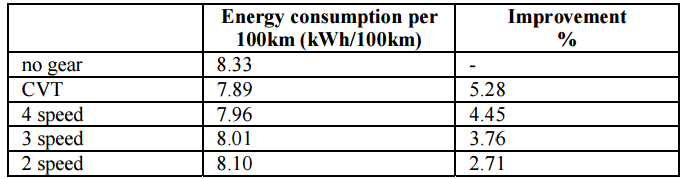
\includegraphics[width=10cm]{fig_1.png}
\caption{\small \sl Efficiency improvements for electric motors for different transmission ratio over the NEDC cycle.}  
\end{figure}

\begin{flushleft}
The recent interest in electric vehicles has however been met with new challenges and trade-offs. The energy density of electric batteries is infinitesimal compared to that of fossil fuels. Pure electric vehicles currently competing in the market are also equipped with single ratio gear transmission, intended to provide a trade-off between efficiency and dynamic performance. However recent research suggests that multi-speed transmission may be employed to provide better dynamic performance without compromising the efficiency that electric vehicles promise.\end{flushleft}

\begin{flushleft}
A prototype for seamless clutch-less two-speed transmission for electric vehicles is already available. The goal of this project is to design and implement control system for this transmission by leveraging real-time industrial controllers that use a holistic approach to gather sensor data pertinent to the immediate surroundings and systematically drive motor speed during gear shifting. Components of the final design must include a National Instruments Compact Reconfigurable IO controller and Arduino Uno microprocessors, and must adhere to CAN serial protocol for communication.\end{flushleft}

\subsection{Final Deliverable}
\begin{flushleft}
This design project, in conjunction with work carried out by another team, is poised towards design and implementation of control system for a two-speed transmission prototype already made available. It is intended that the control system shifts to a different gear ratio by driving the actuators at certain motor speeds, such that the motor speed changes while the output shaft speed keeps at a constant. This project leverages understanding of control systems and modern transmissions to achieve the most desirable outcome.\end{flushleft}

\begin{flushleft}
The final design must include Arduino Uno microprocessors to gather data from the sensor and also actuate transmission solenoids to affect the output gear ratio. The transfer logic of the overall control system is required to be deployed on NI CompactRIO real time controller. The processors must adhere to the vehicle standard CAN serial protocol for communication. Finally the operational system must display real time data on PC screen for diagnostic and acquisition purposes.\end{flushleft}

\subsection{Deliverable Breakdown}
\begin{flushleft}
While still adhering to best practices for design methodologies and keeping with the two-term timeline, the following plan has been devised.
\end{flushleft}

\begin{flushleft}
Term 1: Analysis and Literature Review
\begin{itemize}
  \item Familiarization with theory of control systems, with classical and modern control strategies
  \item Familiarization with LabVIEW and MATLAB environments and languages
  \item Familiarization with relevant communication protocols pertinent to the unit components of final system design 
  \item Initial design and implementation of integrated microcontroller circuit for sensor data acquisition
  \item Implementation and validation of CAN protocol for the microcontroller circuits
\end{itemize}
\end{flushleft}

\begin{flushleft}
Term 2: Design and Validation
\begin{itemize}
  \item Design and validation of controller in the testing environment
  \item Controller implementation in the complete system using LabVIEW programming language and environment
  \item Integration of additional sensors to the microcontroller circuit
  \item Introduction of CompactRIO to the implemented CAN network
  \item Testing and calibration of the sensors and the CAN inter-connect
  \item Testing of the integrated system with the existing testbed
\end{itemize}
\end{flushleft}

\section{Background}
\subsection{CAN communication protocol}
\begin{flushleft}
Controller Area Network (abbreviated as CAN) is an industry standardized in-vehicle communication protocol. It is a message-based serial protocol designed to establish intercommunication between electronic devices and/or micro-controllers in applications without a master controller. In automotive applications such devices include engine management system, anti-lock braking system, gear control system, active suspension, airbags etc. As an example of intercommunication in automobiles – a spark ignition engine requires feedback from the engine control unit to control the precise timing of initiating the combustion chamber in order to provide better fuel efficiency while releasing more power. Similarly a transmission control unit leverages data passed by the engine control unit, the gearbox and various other sensors in the system to change the gear ratio at different speeds.
\end{flushleft}

\begin{figure}[!ht]
\centering 
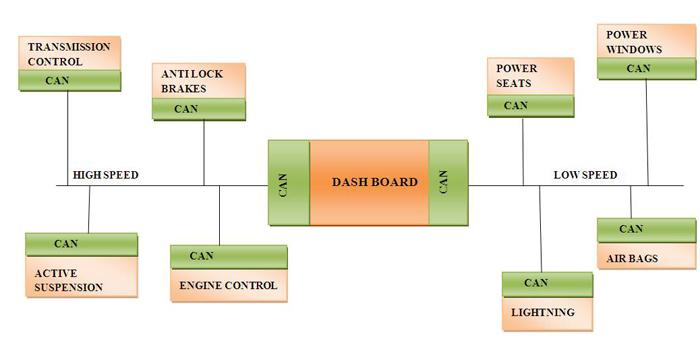
\includegraphics[width=10cm]{fig_2.png}
\caption{\small \sl CAN interconnect layout.}  
\end{figure}

\begin{flushleft}
CAN is characterized as CSMA/CD+AMP protocol [4]. CSMA, or carrier-sense multiple-access protocol means that each node on the bus is required to wait for a prescribed period of inactivity before it can prompt to send a message. CD+AMP, or collision detection and arbitration on message priority states that in the event of collision when multiple nodes prompt to get ownership of the bus, a bit-wise arbitration is carried out based on a pre-programmed priority of each message specified in the identifier field of the message. The CAN standard defines “dominant” bit to be logical 0 and “recessive” bit to be logical 1. Hence a lower corresponding binary value signifies higher priority, thereby leading to winning bus access. By the ISO-11898:2003 standard specification, a standard 11-bit identifier is capable of supporting signaling rates between 125kbps to 1Mbps [4]. Such configuration provides for 211 or 2048 message identifiers.
\end{flushleft}

\begin{flushleft}
Since CAN uses the method of bit-wise arbitration to resolve collision, all nodes on the network are required to sample every bit of data on the bus on the same pulse. During transmission, if one node transmits a dominant bit and another node transmits a recessive bit at the same time, a collision is registered. Arbitration is carried out that grants the node transmitting the dominant bit higher priority for broadcasting. There is no delay to the higher priority message transmission during this arbitration procedure. The node transmitting recessive bit simply attempts re-transmission following six bit clocks interval after the end of the dominant message. 
\end{flushleft}

\begin{figure}[!ht]
\centering 
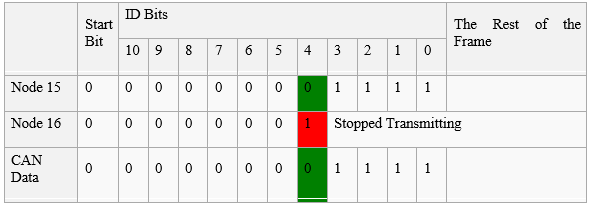
\includegraphics[width=12cm]{fig_3.PNG}
\caption{\small \sl CAN interconnect layout.}  
\end{figure}

\begin{flushleft}
In order to establish CAN communication, each constituent node in the network is required to have a central processing unit, a CAN controller and a CAN transceiver. 
\begin{itemize}
	\item Central processing unit is the host processor that parses messages received over the bus and also decides what message is to be transmitted by the host node. Typically control devices, sensors and actuators are connected to such processing units.
    \item The CAN controller acts as an intermediary buffer which stores the received serial bits from the bus until an entire message worth of bits has been received. The controller then triggers an interrupt following which the host processor may fetch the received data. In the event of broadcasting the host processor sends the message to the controller, which initiates serial bit transmission onto the bus.
    \item The CAN transceiver acts as a message parser while receiving message, converting the received data stream from CAN bus levels to that understandable by the controller; and vice-versa when the node is transmitting. Transceiver also has protective circuitry that shields the controller from possible damage stemming from power surges on the bus line.
\end{itemize}

\begin{figure}[!ht]
\centering 
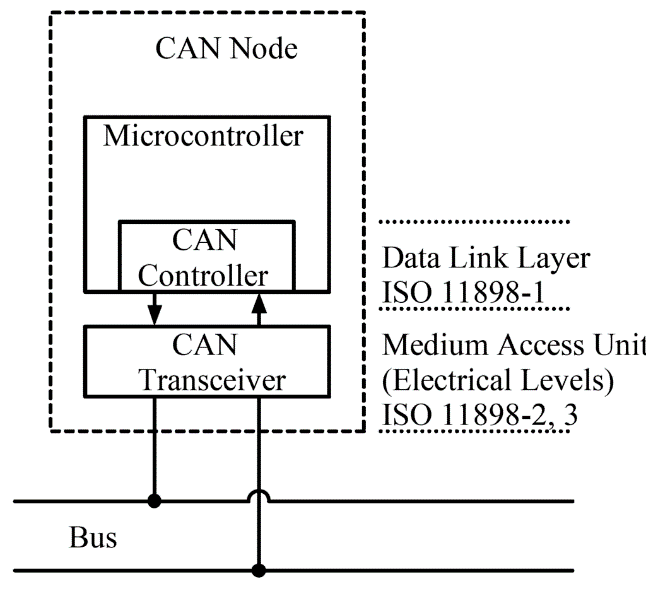
\includegraphics[width=6cm]{fig_4.png}
\caption{\small \sl Anatomy of a CAN node.}  
\end{figure}
\end{flushleft}

\begin{flushleft}
The implementation specific to this project is comprised of a network of two nodes – an Arduino Uno microprocessor and a NI CompactRIO real time controller. Each of these devices have hardware add-ons available that enables them to communicate over CAN. For the Arduino microprocessor a Seeed Studio CAN-BUS V1.2 shield has been acquired. The shield adopts a CAN controller and a CAN transceiver, which can be directly plugged into our Arduino Uno board to provide CAN bus capability. A pluggable NI 9853 High-Speed CAN Module has also been acquired for the NI CompactRIO real time controller, which is connected via the reconfigurable field programmable gate array (abbreviated as FPGA) chassis within the controller.
\end{flushleft}

\begin{flushleft}
The Arduino CAN shield comes equipped with extensive mcp can.h API enablement -– which takes away the minute details of the communication architecture discussed previously and simplifies the implementation. The CAN controller embedded in the Arduino shield however employs Serial Peripheral Interface (abbreviated as SPI) protocol to interface with the host processor – but the SPI.h available library also provides wrapper functions that simplifies implementation. The libraries provide flexibility in implementing standard and extended CAN frame transmission and also provide functionality for transmissions at variable baud rate, hence allowing for flexible and robust programmability. 
\end{flushleft}

\begin{flushleft}
The NI LabVIEW graphical programming environment has been used to implement CAN communication functionality on the real time controller. The programming environment provides the Frame API that simplifies bit-wise processing and manipulation of data transmitted and received on the CAN module at the FPGA level. The Frame Channel Conversion library is also available to enable programming at the real time controller level, which requires conversion of received frames on the CAN module to channels. Thus the supporting API is very well defined for the hardware add-ons acquired for our processors of interest, hence enabling more granular programmability.
\end{flushleft}

\subsection{Transmission Control}
\begin{flushleft}
Control of modern automatic transmission system involves leveraging data gathered from the engine control module and various sensors across the automotive system to calculate the precise gear shift timings. The control system generates output signals that acts upon specialized actuators called transmission solenoids to accomplish this shifting. Modern transmission control systems are further optimized to contribute to improved vehicle performance, better shift quality and higher fuel efficiency – thereby leading to overall reduced engine emissions and greater shift system reliability. Recent advancements in technology also provided for increased programmability of the control system, thereby allowing configurability of transmission characteristics for different automotive applications.
\end{flushleft}

\begin{flushleft}
Transmission control systems operate in close integration with sensors and solenoids to provide a more holistic approach in gear shifting. In a typical control system the sensors register the throttle position, vehicle speed, gear position selection and other different parameters. The information gathered by these sensors are passed to the transmission control module (abbreviated as TCM) which adjusts the current supplied to the transmission solenoids and other specialized controllers to change the effective gear ratio and hence affect vehicle speed.
\end{flushleft}

\begin{figure}[!ht]
\centering 
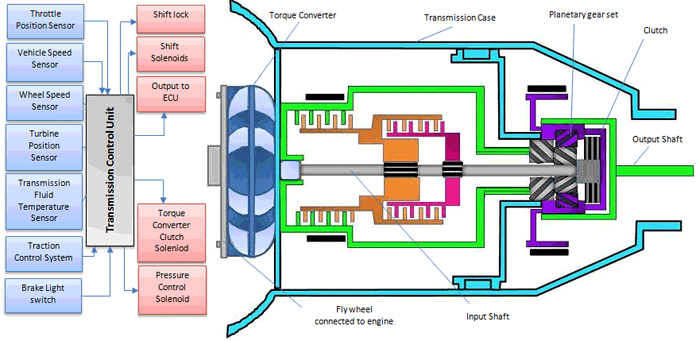
\includegraphics[width=11cm]{fig_5.png}
\caption{\small \sl Sensor-solenoid interfacing via transmission control module.}  
\end{figure}

\begin{flushleft}
Our testbed includes a two-speed clutch-less transmission prototype comprising a dual-stage planetary gear set with common ring and common sun gears [7]. Gear change is accomplished by actuating on two friction brakes that controls the flow of power, hence the speed of the aforementioned gears. Hence gear ratios are toggled by braking either the sun or the ring gears. The friction brakes are actuated by variable force solenoids also provided as part of the system implementation, which in turn are connected to a drive circuit powered by the Arduino microprocessor board. 
\end{flushleft}

\begin{figure}[!ht]
\centering 
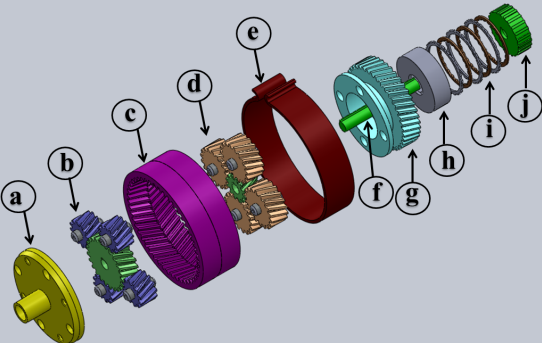
\includegraphics[width=9cm]{fig_6.png}
\caption{\small \sl Exploded view diagram of transmission prototype: a) input carrier b) first stage planetary gear set c) common ring gear d) second stage planetary gear set e) band brake f) common shaft for sun gears g) output carrier h) outer hub for the sun brake i) friction plates j) inner hub for the sun brake.}  
\end{figure}

\subsection{Transmission System Modelling }
\begin{flushleft}
The movement of the two brakes in the transmission system is generated using solenoid actuators. The solenoids are activated by the current passing through them. The function relating the voltage and the current in the solenoid is given in equation 1. The corresponding Laplace domain transfer function is given in equation 2. The state space equations are given in equations 3 and 4, where the output variable y is the current and the control variable u is the current. This is the model for which the control system will be designed. 
\end{flushleft}

\subsection{Control System Design}
\begin{flushleft}
The two brakes will be considered as uncoupled in their transfer characteristics. This means each can be controlled individually as a SISO system. Controlling SISO systems can be achieved using a SISO controller. As the transfer function for the current in the solenoids is linear, it can be controlled using a linear controller. This leads to the full control system model shown in Figure 8.\end{flushleft}

\begin{figure}[!ht]
\centering 
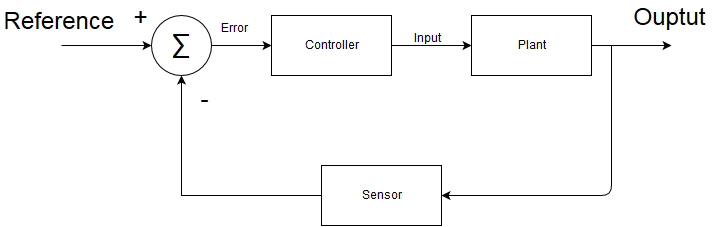
\includegraphics[width=10cm]{fig_7.png}
\caption{\small \sl Exploded view diagram of transmission prototype: a) input carrier b) first stage planetary gear set c) common ring gear d) second stage planetary gear set e) band brake f) common shaft for sun gears g) output carrier h) outer hub for the sun brake i) friction plates j) inner hub for the sun brake.}  
\end{figure}

\begin{flushleft}
Classical control techniques include algorithms and strategies for choosing the components of linear controllers. These are often chosen to have three terms; proportional to the error, to the derivative of the error and to the integral of the error. The proportionality coefficients are chosen for the system to satisfy given criteria about characteristics of the complete system, including steady-state error, stability, robustness and bandwidth. Other possible characteristics include rise time, settling time and boundedness of the controller output. All of these can be verified by MATLAB simulations.\end{flushleft}


\section{Requirements}
\begin{flushleft}
The goal of this project is to control the gear-shifting mechanism by controlling the brakes. As explained previously, the behavior of the brakes themselves is dictated by the current flowing through the solenoid. This is therefore the variable to be controlled with the input voltage, as given in equations 3 and 4. Each actuator will be controlled with a PID controller. The proportionality constants for each term will be adjusted to provide optimal closed loop behaviour of the complete system. The design will include justification for balancing robustness and a quick response. 
\end{flushleft}

\begin{flushleft}
The controller will be software defined and will execute on the CompactRIO. The implementation of the controller will be achieved using the LabVIEW environment. To ensure the most efficient implementation of the controller, the use of ready-made components such as integrators will be limited. These will have to be as computationally efficient as permitted by the language. This choice of implementation requires familiarity with the programming environment. 
\end{flushleft}

\begin{flushleft}
The controller may be placed physically distant from the input to the actuators. Therefore, the control signal is sent by CAN bus to an Arduino, which models an electrical control unit in the final model of the system. The control signal can then be locally amplified and transmitted to the actuator. Sensors, powered by another Arduino, will measure data from the output of the system and send it back to the CompactRIO, thus allowing for the closed-loop control of the system. This system is shown in figure 9.
\end{flushleft}

\begin{figure}[!ht]
\centering 
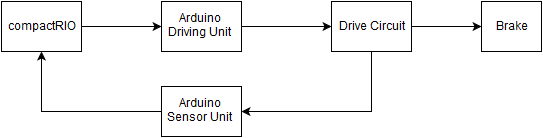
\includegraphics[width=11cm]{fig_8.png}
\caption{\small \sl System Implementation.}  
\end{figure}

\begin{flushleft}
The communication protocols used between the Arduinos and the CompactRIO, as well as the hardware-based limitations of each individual component, will set limitations on the operating frequency of the complete system. For example, the CAN protocol establishes operating frequencies between 125 kbps to 1 Mbps. Most of the components allow for programmable operating frequencies, so the exact values will be determined as the project progresses. 
\end{flushleft}

\section{Design and Results}
\subsection{Control System Design}

\begin{flushleft}
The design of the controller and its implementation were separated into two components. The design aspect will be conducted using MATLAB tools, while the implementation will be fully achieved with LabVIEW. The use of MATLAB permits the automated and simplified study of the characteristics of the system. Several goals were established for this semester in control system design. 
\end{flushleft}

\begin{itemize}
	\item Study of control theory
    \item Familiarity with MATLAB
    \item Familiarity with LabVIEW
\end{itemize}

\begin{flushleft}
Firstly, familiarity with MATLAB was achieved through the implementation of a simple control system for a plant with the same transfer function as the solenoid. Simulations were run for different parameter values and several integrated tools with later utility were explored. The model used is shown in figure 9. The step response of the system, after having tuned the PID controller using the PID controller tuning tool in SIMULINK, is shown in figure 10. Establishing SIMULINK as a tool to be used in the design and validation of the controller simplifies the tasks by allowing the simulation of parameterized systems for many sets of values.
\end{flushleft}

\begin{figure}[!ht]
\centering 
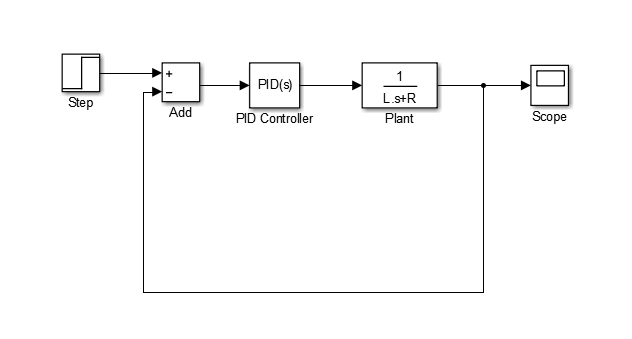
\includegraphics[width=11cm]{fig_9.png}
\caption{\small \sl Simulink Implementation of PID controller.}  
\end{figure}

\begin{figure}[!ht]
\centering 
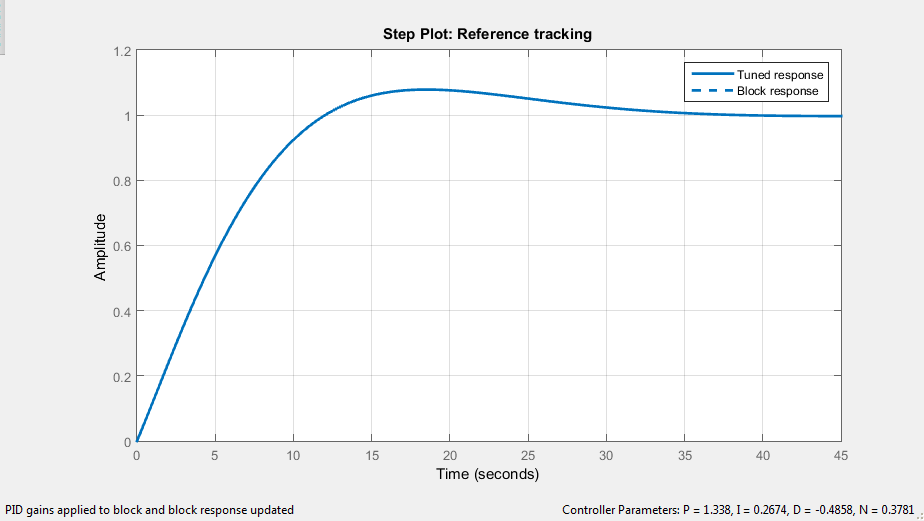
\includegraphics[width=11cm]{fig_10.png}
\caption{\small \sl Step Response of Tuned Circuit.}  
\end{figure}

\begin{flushleft}
To ensure adequate familiarity with the LabVIEW language and environment, two tools were designed. The first tool takes as input the transfer functions of the plant and of the controller. It then computes the closed-loop transfer function of the system and simulates and graphs the step response. The second tool simulates the step response to a block diagram realization of a PID controller. 
\end{flushleft}

\begin{flushleft}
To finalize the familiarization phase, a naïve implementation of a PD controller was achieved. The controller used the first difference of the input error as the derivative term. This implementation of the controller demonstrates the basic techniques expected to be used in the later versions of the design, instead of validating the controller configuration or tuning. These include the use of shift registers as memory elements from which to generate derivatives and integrators. 
\end{flushleft}

\subsection{System Module Integration}
\begin{flushleft}
The overall system design implements two Arduino Uno microcontrollers intended for sole purposes of sensor data acquisition and solenoid actuation. This phase of the design process imposes hardware resource constraints required for implementation and testing. The design task has been condensed into implementing only one microcontroller integrated circuit for this semester – in specific the sensor data acquisition circuit. With time and available hardware resource permitting, it has been planned to additionally implement and validate CAN communication protocol between the two microcontrollers. The intended deliverables for this semester can be summarized as follows:
\end{flushleft}

\begin{itemize}
  \item Familiarization with relevant communication protocols pertinent to the unit components of the overall network system
  \item Initial design and implementation of sensor integrated microcontroller circuit
  \item Implementation and validation of CAN protocol between the microcontroller circuits
\end{itemize}

\begin{flushleft}
The initial implementation of the microcontroller circuit has been carried out with an atmospheric pressure click sensor. This necessitated familiarization with the associated communication protocol employed by the sensor, namely I2C. Owing to being the first Arduino coding exercise, a more rigorous coding approach has been followed to provide thorough and conclusively functional circuit. Some of the key implementation details have been further discussed below, complemented with code snippets. All Arduino developments have been carried out using the Arduino IDE, the official supporting integrated development environment. The code extensively refers to the register values specified in the pressure sensor datasheet. In details that follow, the Arduino Uno microcontroller is considered the master and the pressure click sensor considered the slave. The Arduino Wire library has been used to establish the I2C communication.
\end{flushleft}

\begin{figure}[!ht]
\centering 
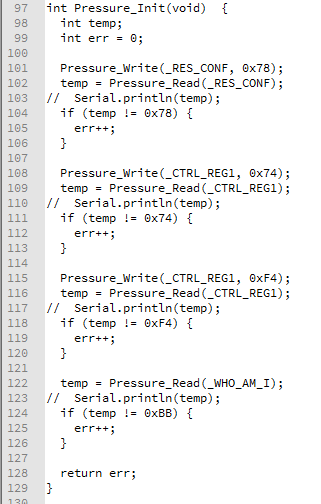
\includegraphics[width=6cm]{1.png}
%\caption{\small \sl Step Response of Tuned Circuit.}  
\end{figure}

\begin{flushleft}
The first code snippet shows the initial setup phase of the slave circuit. This routine is intended to run only once during circuit boot-up. The master first configures the resolution for the pressure gauge by setting specialized register bits. The routine also initializes control register bits to select the output data rate for the sensor, followed by rebooting the sensor chip for the changes to take effect. Several debugger statements have been intermittently placed in the code to ensure that correct values have been passed to the registers during this setup process. Finally as part of error checking mechanism, register read backs have been implemented to check whether the values found matches as previously specified. 
\end{flushleft}

\begin{figure}[!ht]
\centering 
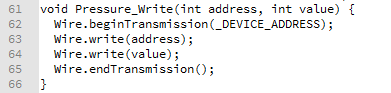
\includegraphics[width=6.4cm]{2.png}
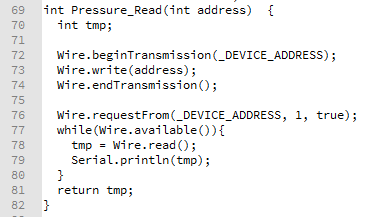
\includegraphics[width=6.4cm]{3.png}
%\caption{\small \sl Step Response of Tuned Circuit.}  
\end{figure}

\newpage
\begin{flushleft}
The code snippet to the left specifies Arduino implementation of the I2C write protocol. This routine is called during the sensor initialization phase to set the register values. As a background on I2C, following instruction sequence can be considered during a write event:
\end{flushleft}

\begin{itemize}
\item Sending a start sequence
\item Sending slave address with R/W bit low (even address)
\item Specifying internal register that needs to be written to
\item Sending data bytes
\item Stopping sequence
\end{itemize}

\begin{flushleft}
Implementing particularly the 2nd instruction in the sequence specified by the I2C protocol presented challenges. Initial iterations of the code first manipulated the slave device address to set the R/W bits accordingly for a write operation. This however failed to boot-up and initialize the sensor once the associated routine is called. The debugger and error checking statements proved to be effective during this exercise. 
\end{flushleft}

\begin{flushleft}
The code snippet on the right shows Arduino implementation of the I2C read protocol. Depending on the resolution and data rate specified during initialization, specialized slave register values are set, that are read back periodically by the master to report the final sensor reading. The I2C protocol adheres to the following sequence of instructions for a read operation:
\end{flushleft}

\begin{itemize}
\item Sending a start sequence
\item Sending slave address with R/W bit low (even address)
\item Specifying internal address of the bearing register
\item Resending start sequence (also called repeated start)
\item Sending slave address with R/W bit high (odd address)
\item Reading data bytes
\item Stopping sequence
\end{itemize}

\begin{flushleft}
The read operation also imposed additional implementation challenges. In specific, the Arduino Wire library does not have any supported functions for doing repeated start operation (referring to 4th instruction). Failure to implement this routine during initial iterations have been further proved by the debuggers and error checkers planted in the initialization routine. 
\end{flushleft}

\begin{flushleft}
Further testing and analysis showed that both the read and write implementations are simplified using the Wire library. In specific, the Wire library simplifies the bit-masking operations required by I2C to simply transmitting the device address without the R/W bit, and then call Wire.read() and Wire.write(). 
\end{flushleft}

\begin{flushleft}
Following the initial implementation of the data acquisition circuit, CAN communication protocol was established between the two Arduino microcontrollers. Despite the system setup not being representative of the overall design, this exercise was purposefully proposed as a stepping stone that would guide the overall system setup during the next term. The communication was established with the aid of CAN-bus shield and the associated API mcp can.h. Some of the key implementations have been further discussed in the following. 
\end{flushleft}

\begin{figure}[!ht]
\centering 
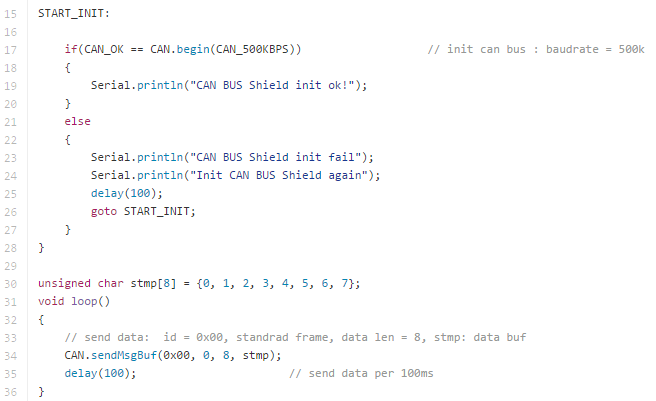
\includegraphics[width=9cm]{4.png}
%\caption{\small \sl Step Response of Tuned Circuit.}  
\end{figure}

\begin{flushleft}
The first snippet of code shows the Arduino implementation for sending CAN messages. The code makes extensive reference calls to helper functions in the API. The first set of instructions initializes the bus and specifies the transmission baudrate. Sending a CAN message involves calling CAN.sendMsgBuf(INT8U id, INT8U ext, INT8U len, data buf) routine, which takes as parameter the length of the message frame, specifier for standard or extended frame length and the data bytes. 
\end{flushleft}

\begin{figure}[!ht]
\centering 
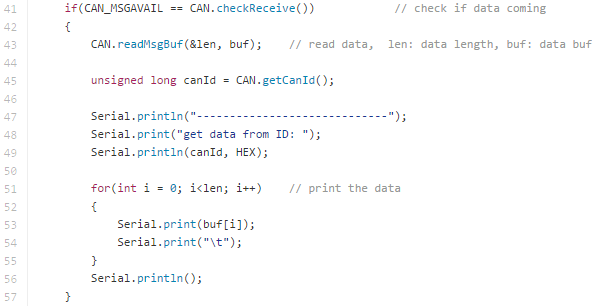
\includegraphics[width=9cm]{5.png}
%\caption{\small \sl Step Response of Tuned Circuit.}  
\end{figure}

\begin{flushleft}
The second snippet of code shows the Arduino implementation for receiving CAN messages. The CAN.checkReceive() polls for received frames. Once a message receive has been registered, the message is written to a predefined buffer using the CAN.readMsgBuf() routine. The received message has been checked with that sent by the initiating node for verification. CAN.getCanId() routine call returns the sender node’s identity, which further verifies the integrity of the communication link.
\end{flushleft}

\section{Plan for next Semester}
\subsection{Full System Integration}
\begin{flushleft}
The current CAN implementation will be extended to bridge the gap between CompactRIO and Arduino. A template for implementation on the CompactRIO FPGA target has been devised at the time of writing this report, which will be used as a guideline in the subsequent term. The existing Arduino - sensor integrated circuit will be extended to include force and altitude sensors to reflect the intended system setup. System data will also be logged real time on the LabVIEW interface front panel for diagnostic/acquisition purpose. 
\end{flushleft}

\subsection{Controller Design and Implementation}
\begin{flushleft}
After sufficient study of control theory and of the relevant classical control techniques, the controller will be designed and validated using MATLAB. Several possible configurations will be verified and tested. Precise characteristic requirements will be established. The expected characteristics will be checked and further optimized. 
\end{flushleft}

\begin{flushleft}
The implementation of the controller will be achieved using LabVIEW software; the constraints of the software on the possible configurations will be taken into account. 
\end{flushleft}

\begin{flushleft}
Once the controller is implemented, it will be tested with a simulated plant. Once accepted as sufficiently robust, the controller will be tested with the actual testbed. 
\end{flushleft}

\section{Impact on Society and Environment}
\begin{flushleft}
The development of electric vehicles has been carried out with a relatively narrow focus as manufacturers have eschewed the multi-speed transmission in favour of a simpler and lighter, single speed transmission. 
\end{flushleft}

\begin{flushleft}
There is a significant gain in range that can be covered by the limited battery supply due to the increase in motor efficiency from keeping the motor in a pre-determined ideal RPM range based on its speed. However, the current ease in balancing an electric motor when compared to an internal combustion engine has hindered the inclusion of a multi-speed transmission.
\end{flushleft}

\begin{flushleft}
Possible advantages of this strategy include:
\end{flushleft}

\begin{itemize}
  \item an increase in up to 20\% in range of an electric vehicle by posing lesser of a burden on the battery when driving at highway-speeds
  \item a dramatic increase of up to 30\% in initial acceleration by means of using a lower-gear ratio for starting which multiplies torque
  \item an easily noticeable increase in top speed by the motor offering increased power in mid-range RPM
  \item a massive reduction in heat emissions as the motor moves to a more efficient RPM range in a much faster fashion which in turn reduces inrush current and energy losses in the form of motor heat.
\end{itemize}

\begin{flushleft}
The above-mentioned improvements can help in greatly increasing the viability of electric vehicles to consumers, especially those who have been hesitant to use them due to a majority of their commutes being at highway-level speeds and distances. Hence, environmental benefits that follow directly from the increased use of electric vehicles instead of the conventional internal combustion engines are aimed to be achieved as a result of this project.
\end{flushleft}

\begin{flushleft}
The environmental impact of making electrical vehicles is greater than that for making gas and diesel vehicles, but this is more than made up for by the greater impact of gas and diesel vehicles while they’re being used. This is true in terms of total energy combustion, use of resources, greenhouse gases, and ozone pollution. Studies have shown that this benefit is obtained even considering the factor of electrical vehicles being assumed to be charged from a grid that includes a significant amount of fossil fuels – they beat gas-powered ones in terms of greenhouse gas emissions even if they’re charged in regions that depend heavily on coal. As an example, a study done by Renault has been referred to that details and compares lifecycle assessments of the battery-electric and two internal combustion engine versions of its sedan, ‘Fluence’ [9]. Just the difference in the carbon footprint (with both, French and UK grid mixes) is highlighted by the figure below.
\end{flushleft}

\begin{figure}[!ht]
\centering 
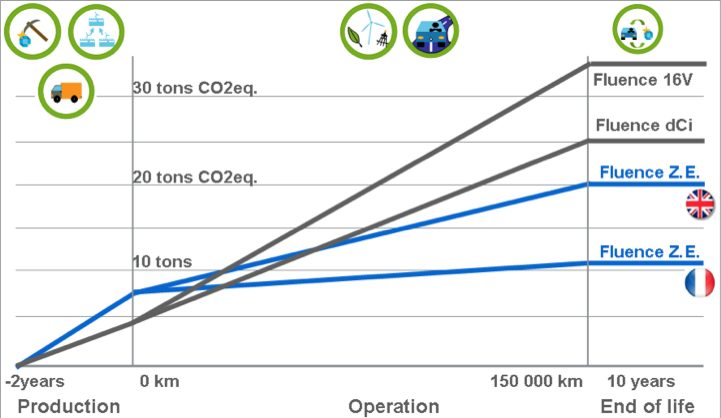
\includegraphics[width=10cm]{fig_11.png}
\caption{\small \sl Comparison of Carbon footprint of EV and ICE versions of Renault Fluence sedan over production, operation and end of life. (Engines: Diesel – 1.5L dCi (66kW), Gasoline – 1.6L 16v (81kW), Electric – 70kW).}  
\end{figure}

\begin{flushleft}
Electric vehicles, coupled with clean and sustainable electricity, are important parts of the solution that meets the challenge of climate change and the increasing dependence on oil. Studies have shown owners of an electric vehicle to save up to 6000 gallons of gasoline [10] which is a massive contribution to any nation’s energy security. Unless electrical vehicles become a market success, which cannot be accomplished without appealing to those who need their vehicles to efficiently commute on highways, significant reductions in the transport sector’s emissions and oil consumption cannot be achieved. 
\end{flushleft}

\begin{flushleft}
It is also important to mention here that from the beginning of the project, it has been made clear that the safety and robustness of the designs is the ultimate concern. Transmission system failures can be catastrophic, so the design of their controllers must account for this need. The requirements take this into account through the desired robustness and stability characteristics of the controller. 
\end{flushleft}

\section{Report on Teamwork}
\begin{flushleft}
This term, the work was primarily divided into tasks relevant to designing the controller and studying the implementation environment, tasks relevant to communication and integration of the individual modules, and organizational and management tasks. The organizational tasks included delegating the work items, liaising with the supervisors and moderating team meetings. Due to the team members’ lack of experience with most of the relevant tools and systems, the organization of familiarization tasks also needed to be organized. The other tasks were as previously described in the report.
\end{flushleft}

\begin{flushleft}
For next term, the delegation of tasks will require reorganization based on the change in focus to system level integration and testing. 
\end{flushleft}

\section{Conclusion}
\begin{flushleft}
This term, the work accomplished shows that the design required is indeed possible and realizable. The first modules that will be used, the Arduino units, were set up and their interactions planned and specified. The controller form was specified and studied. The tools that will be used for the next semester were studied and used. Next term, the focus will be on implementation tasks, integration of all modules and system testing both with a simulated plant and with the existing testbed. 
\end{flushleft}

\begin{flushleft}
Over the course of this project, the importance of parameterizing the designs to be resistant to the inevitable changes that occur over the course of a full process was realized. Such a parameterization includes specifying model inaccuracies, protocol flexibility and sensor calibration specifics. Designing for unknown parameters in each of these characteristics was not easy but allowed us to keep a working version of each design as the specifications evolved. 
\end{flushleft}


\end{document}